\documentclass[11pt]{article}
\pdfinfoomitdate=1
\pdftrailerid{}
\pdfsuppressptexinfo=15
\usepackage{fullpage,amsmath,amssymb,amsthm}
\usepackage[T1]{fontenc}
\usepackage{lmodern}
\usepackage{graphicx}
\usepackage[title]{appendix}
\usepackage{url}
\usepackage[colorlinks=true,linkcolor=blue,citecolor=blue,urlcolor=blue]{hyperref}
\hypersetup{pdftitle={Sharp linear bounds for the EKG sequence},
  pdfauthor={P. Graham},
  pdfsubject={Integer sequences and formalized mathematics},
  pdfkeywords={EKG sequence, greedy permutation, explicit bounds, large sieve, Lean}}
\newtheorem{theorem}{Theorem}
\newtheorem{proposition}[theorem]{Proposition}
\newtheorem{lemma}[theorem]{Lemma}
\newtheorem{corollary}[theorem]{Corollary}
\theoremstyle{definition}
\newtheorem{definition}[theorem]{Definition}
\theoremstyle{remark}
\newtheorem{remark}[theorem]{Remark}
\newcommand{\U}{U}
\newcommand{\spf}{\operatorname{spf}}
\newcommand{\piU}{\pi^{+}}
\newcommand{\piL}{\pi^{-}}
\newcommand{\lean}[1]{\texttt{#1}}
\title{Sharp linear bounds for the EKG sequence}
\author{P. Graham\\ \small\url{https://orcid.org/0009-0007-8493-1505}}
\date{October 26, 2026}
\begin{document}
\maketitle

\begin{abstract}
We prove that the EKG sequence satisfies $13n/28\le a(n)\le12n/7$ for
every $n\ge1$, with equality only at $n=28$ and $n=7$, respectively.
Discovered by Jonathan Ayres, the sequence starts with $1,2$ and
repeatedly takes the least unused
positive integer sharing a factor greater than $1$ with its predecessor.
This proves the sharp linear bounds conjectured by Lagarias, Rains and
Sloane, who established coarse bounds at every index. Hofman and Pilipczuk
proved the limits $1/2$, $3/2$ and $1$ of $a(n)/n$ on primes, their
triples and the other terms, and Haver made these estimates explicit and
formalized them in Lean. Our earlier
second-order asymptotic also builds on Haver's work. We sharpen Haver's
self-improving early-even bound with a shorter prime window and effective
large-sieve constants, and control odd terms so that the analytic range
meets a finite computation. Lean checks the deduction from
the definition, conditional on computed premises; independent programs
check those premises, and their correspondence with the formal
statements was checked by reading the code.
\end{abstract}

\begin{quotation}\small\noindent
This work has not yet been reviewed by experts.
The proofs, the Lean formalization, the programs and the text were
produced by AI models (from OpenAI and Anthropic), working under the
author's direction.
\end{quotation}

\bigskip
\noindent 2020 \emph{Mathematics Subject Classification}:
Primary 11B83; Secondary 11N36, 68V15.\\
\emph{Keywords}: EKG sequence, greedy permutation, explicit bounds,
large sieve, formal verification.




\section{Introduction}

The EKG sequence, discovered by Jonathan Ayres and studied by Lagarias,
Rains and Sloane \cite[Introduction]{lrs},
is \href{https://oeis.org/A064413}{A064413} in the OEIS \cite{oeis}.
Write $\U_t=\{a(1),\dots,a(t)\}$. The sequence is defined by
\begin{equation}\label{eq:rule}
 a(1)=1,\quad a(2)=2,\quad
 a(n)=\min\{m\ge1:\ m\notin\U_{n-1},\ \gcd(m,a(n-1))>1\}\quad(n\ge3),
\end{equation}
so it begins $1,2,4,6,3,9,12,8,10,5,15,18,14,7,21,24,16,20,22,11,\dots$.
It is a permutation of the positive integers \cite[Theorem~1]{lrs}
(Theorem~2.5 in the journal version).
Its graph has three visible lines (Figure~\ref{fig:ratio}): most terms
satisfy $a(n)\approx n$, while each odd prime $p$ is immediately preceded
by $2p$ and followed by $3p$, and when $a(n)=p$ we have $p\approx n/2$
(and $a(n+1)=3p\approx3n/2$).
Lagarias, Rains and Sloane proved $n/260\le a(n)\le 14n$ and
conjectured sharp linear bounds \cite[Conjecture~3, end of \S4]{lrs}
(Conjecture~4.3 in the journal version):
\begin{quote}
\emph{The sequence $a(n)$ satisfies $a(n)\ge\frac{13}{28}n$, with
equality if and only if $n=28$, and $a(n)\le\frac{12}{7}n$, with
equality if and only if $n=7$.}
\end{quote}

\begin{theorem}\label{thm:main}
For every integer $n\ge1$,
\[
 \frac{13}{28}\,n\ \le\ a(n)\ \le\ \frac{12}{7}\,n .
\]
The lower bound is an equality only for $n=28$ (where $a(28)=13$) and the
upper bound only for $n=7$ (where $a(7)=12$).
\end{theorem}

\begin{figure}[t]
\centering
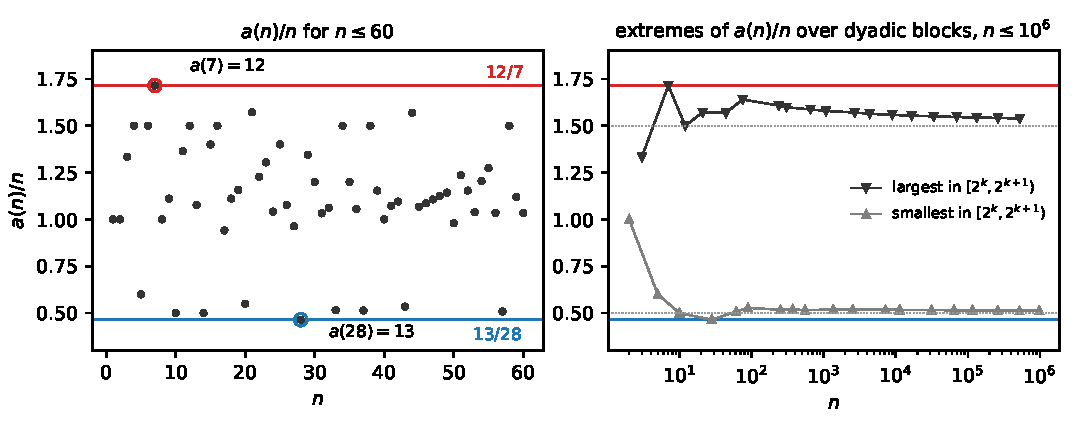
\includegraphics[width=\linewidth]{../data/ratio.pdf}
\caption{Left: $a(n)/n$ for $n\le60$, with the bounds $12/7$ (top) and
$13/28$ (bottom) of Theorem~\ref{thm:main}, attained at $n=7$ and $n=28$.
Right: the largest and smallest values of $a(n)/n$ over each block
$2^k\le n<2^{k+1}$, $n\le10^6$, approaching $3/2$ and $1/2$ (dotted).
Drawn from the computed sequence.}
\label{fig:ratio}
\end{figure}

\paragraph{Prior work.}
Lagarias, Rains and Sloane give the pointer rule as an alternative
definition \cite[eq.~(2)]{lrs} and prove the coarse bounds above
\cite[Theorems~2--3]{lrs}. Their Conjecture~2 states
$a(n)\sim n(1+1/(3\log n))$ when $a(n)$ is neither $p$ nor $3p$ for a
prime $p$, $a(n)\sim(n/2)(1+1/(3\log n))$ when $a(n)=p$, and
$a(n)\sim(3n/2)(1+1/(3\log n))$ when $a(n)=3p$ \cite[Conjecture~2]{lrs}.
Hofman and Pilipczuk
\cite[Theorems~4.3, 4.17, Lemma~4.5 and Corollary~4.12]{hp} proved the full pattern
$2p,p,3p$ for odd primes, bounded the crossings of a level by composite terms,
and proved the leading limits $a(n)/n\to1/2$, $3/2$ and $1$ for prime,
triple-prime and remaining terms, respectively. Haver made these arguments
explicit and formalized them in Lean
\cite[(F2), Theorems~5, 8, 11 and Corollary~12(b)]{haver},
reducing the pattern's computed base to the primes $p\le43$, bounding the
number of used even numbers above the least missing even number, the
spread of the terms above it, and the unused composites below it, and relating the index to
that even number by a counting identity. The author \cite{graham}
then obtained a second-order asymptotic, $n+n/(3\log n)+o(n/\log n)$, for
a smoothed version of the sequence (each odd prime $p$ and $3p$ replaced by $2p$),
on Haver's Lean foundation. The present proof uses Haver's Lean
definition of the sequence and Haver's estimates, and the author's exact form
of the counting identity, as proved Lean theorems.

Haver already closes a self-improving early-even inequality and obtains
its leading asymptotic constant by Brun--Titchmarsh
\cite[Lemma~4, Theorem~5, Remark~6(b)]{haver}. The hardest step is to make
that inequality close at a frontier reached by a finite computation;
Haver's explicit bound is too weak at that frontier. We shorten the
prime window from $4K+3$ to $3K+2$ integers, where $K$ counts the used
even numbers above the least missing even number; effective large-sieve constants
and odd-term control make the analytic range meet a finite computation.

The proof uses Lean and computations of a finite prefix and an
interval-arithmetic certificate. Section~\ref{sec:trust} gives the formal
statement and its relation to the theorem; Appendix~\ref{app:checks}
describes the computed premises and their checks.

 The result is computer-assisted. 

\section{Notation and known facts}\label{sec:notation}

All logarithms are natural. The notation below separates the three kinds
of terms and the errors
in the counting identity. The terms \emph{frontier}, \emph{early evens} and \emph{tick value}
follow Haver \cite[\S\S1--2]{haver}.
A \emph{state} $t\ge1$ is the moment after $a(1),\dots,a(t)$ have been
placed. For a state $t$ define:
\begin{itemize}
\item $E(t)$, the \emph{frontier}: the least positive even integer not in
  $\U_t$. It is nondecreasing in $t$, and every even number below $E(t)$
  is used.
\item $K(t)$, the number of \emph{early evens}: even $w\in\U_t$ with
  $w>E(t)$.
\item $B_q(t)$, the least multiple of $q$ not in $\U_t$.
\item A \emph{tick value} is $3p$ with $p$ an odd prime. $T(t)$ is the
  largest element of $\U_t$ that is not a tick value, and $O(t)$ is the
  number of odd $w\in\U_t$ with $w>E(t)$ that are not tick values.
\item $H(t)$, the number of \emph{holes}: composite $h<E(t)$ with
  $h\notin\U_t$.
\item $A(x)=\pi(x)-2\pi(x/2)+\pi(x/3)$, where $\pi$ counts primes.
\end{itemize}
For example, after $a(1..7)=1,2,4,6,3,9,12$ we have $E(7)=8$, the early
even $12$, so $K(7)=1$, and $O(7)=0$ since $9$ is a tick value.

We use the following facts; each is a Lean theorem in the foundation
(Section~\ref{sec:trust}). The parenthesized labels refer to the
statements recalled here.

\begin{itemize}
\item[(F1)] \emph{Pointer rule} \cite[eq.~(2)]{lrs}. $a(n)=\min\{B_q(n-1):q\text{
  prime},\ q\mid a(n-1)\}$ for $n\ge3$.
\item[(F2)] \emph{Prime pattern.}
  For each odd prime $p$ there is an index $N_p$ with $a(N_p)=2p=E(N_p-1)$,
  $a(N_p+1)=p$ and $a(N_p+2)=3p$; the value $3p$ occurs only at $N_p+2$,
  and indices $N_p$ of distinct primes differ by at least $4$.
  See \cite[Theorem~4.3]{hp} and \cite[(F2)]{haver}; the finite checks and
  detailed attributions are in Appendix~\ref{sec:finite}.
\item[(F3)] \emph{Crossings} \cite[Lemma~4.5]{hp}, \cite{haver}. For a
  level $x>2$, at most $\pi(\sqrt x)$ indices $n$ have $a(n)$ composite and
  $a(n)<x\le a(n+1)$.
\item[(L7)] \cite[Lemma~7]{haver} $B_3(t)\le E(t)+6K(t)+6$ for $t\ge9$.
\item[(SP)] \emph{Span} \cite[Theorem~8]{haver}. With $k=K(t)+1$ and
  $e=E(t)$, $T(t)-e\le 2k^2+2k\sqrt{k^2+e}$ for $t\ge9$.
\item[(EE)] Our variant of \cite[Lemma~4]{haver}, from its proof. Call $i<t$ a \emph{prime up} at state
  $t$ if $a(i)$ is prime and $a(i)<E(t)\le a(i+1)$; it is \emph{paired} if
  $a(i+1)$ is odd and $a(i+2)<E(t)$, and \emph{unpaired} otherwise. Then
  $K(t)\le\pi(\sqrt{E(t)})+1+\#\{\text{unpaired prime ups at }t\}$.
  Pairing uses only terms already placed at state $t$, so $i+2\le t$ is
  required; a prime up with $i+1=t$ is unpaired.
\item[(CL)] \emph{Counting identity} \cite[Corollary~12(b)]{haver}, in the exact form of
  \cite{graham}. For $t\ge9$ and $e=E(t)$,
  \[ e-t=A(e)+H(t)-K(t)-O(t)+c(t),\qquad 1\le c(t)\le5 .\]
\end{itemize}

Here $c(t)$ is the bounded correction in (CL). A crossing of a level
is a step from one side of that level to the other; upward and downward
refer to its direction. The inequalities in (F3) fix the convention at
an endpoint.

Write $\piL(x)\le\pi(x)\le\piU(x)$ for the explicit prime-counting
bounds in Appendix~\ref{app:prime}; $\pi(x)$ counts primes up to $x$.
The following two forms of the large sieve are proved in Lean.
\begin{itemize}
\item[(BT)] \emph{Primes in short intervals.} For real $x>0$, $y\ge1$ and
  integers $Q\ge6$,
  \[\pi(x+y)-\pi(x)\le\frac{y+Q^2}{\log(Q+1)+1.07}+\pi(Q).\]
  We use the additive inequality of Montgomery and Vaughan
  \cite[Theorem~1]{mv} and their arithmetic lower bound
  \cite[(2.7)]{mv}, which they credit to Montgomery \cite{montgomery}.
  OpenAI's formalization \cite{oaimath} already supplies the arithmetic
  large sieve with Farey separation $1/Q^2$. For (BT) we use separation
  $1/(Q^2-1)$ to obtain the numerator $y+Q^2$. We also prove
  $G(Q)=\sum_{d\le Q}\mu^2(d)/\varphi(d)>\log(Q+1)+1.07$, the form
  in the proof of \cite[Lemma~7]{mv}, whose printed statement is
  $G(z)\ge\log z+1.07$ for real $z\ge6$.
\item[(LS)] \emph{Arithmetic large sieve} \cite{montgomery,mv}. For an integer $Q\ge2$, a set of
  integers in an interval of $N$ consecutive integers that avoids one
  residue class modulo every prime $p\le Q$ has at most
  $(N+Q^2)/\log Q$ elements.
\end{itemize}

\section{Strategy}\label{sec:overview}

The three kinds of terms behave differently, and each is located through
the frontier. If $a(n)=p$ is an odd prime then $n=N_p+1$ and $E(n-2)=2p$
by (F2); if $a(n)=3p$ then $n=N_p+2$ and $E(n-3)=2p$; every other term
either lies above the frontier $E(n-1)$, and then at most $T(n)$, or
fills a hole below it, and holes lie close to the frontier. The counting identity (CL) relates the index $t$ to $e=E(t)$:
$A(e)\approx e/(3\log e)$ is small, and if $K$, $O$ and $H$ are small
compared to $e$, then $t\approx e$ and the three kinds of terms give
$a(n)/n$ near $1/2$, $3/2$ and $1$.

Everything therefore rests on explicit upper bounds for $K$, $O$ and $H$
at every state, uniformly in a range of $e$. Haver bounds each by a
multiple of $\pi(\sqrt e)$ (times further factors), so the bounds are
relatively small only when $e$ is astronomically large. We split the
indices into three ranges:
\begin{enumerate}
\item $n\le L=1.6\cdot10^{10}$: computed (Section~\ref{sec:finite});
\item $L<n<10^{203}$: a bootstrap bound $K(t)\le M(E(t))$ for a step
  function $M$, certified with $E(L-2)\ge e_0=1.3328\cdot10^{10}$ and on
  every interval of a cover of $[e_0,10^{205})$ (Sections
  \ref{sec:K}--\ref{sec:middle});
\item $n\ge10^{156}$: Haver's bounds alone (Section~\ref{sec:far}).
\end{enumerate}
The ranges overlap, so every $n$ is covered. Range~2 requires the bound
on $K$ already at $e=1.3328\cdot10^{10}$.

\paragraph{The early-even bound.}
Theorem~\ref{thm:main} needs sharp constants at every $n$: the lower line
$a(n)/n\to1/2$ sits only $1/28$ above $13/28$. With Haver's bound
$K\le12\pi(\sqrt E)+720$ \cite[Theorem~5]{haver} the argument closes
only for very large $n$; we use it that way for $n\ge10^{156}$
(Lemma~\ref{lem:F}), far beyond any computation.
The quantitative improvement uses a shorter prime window
(Lemma~\ref{lem:A}, Corollary~\ref{cor:A}): the primes responsible for
the excess of $K$ lie among the $3K+2$ integers just below $E/2$, so
$K\le\pi(\sqrt E)+2+\#\{\text{primes among }3K+2\text{ consecutive integers}\}$, and a
Brun--Titchmarsh bound from the large sieve turns this into
$K\le(1+o(1))\pi(\sqrt E)$. The bound is proved by induction over the
moments of the sequence, so it needs no prior bound on $K$: at each moment
the earlier ones already satisfy it, and an explicit inequality, checked
on intervals of $E$, carries it to the next. At $E=1.3328\cdot10^{10}$
the certified bound is $28{,}017$, against $131{,}628$ from Haver's bound.
A second
large-sieve bound controls the odd terms above $E$ (Lemma~\ref{lem:D}).
With these, explicit estimates close once $E\ge1.3328\cdot10^{10}$; the
computed first $1.6\cdot10^{10}$ terms reach that point (with $E$ above
$1.41\cdot10^{10}$ by $n=1.393\cdot10^{10}$) and settle every smaller $n$.

\section{Early evens}\label{sec:K}

We bound the primes responsible for early evens. For a state $t$ let
$K^{<}(t)=\max\{K(s):1\le s<t\}$, with $K^{<}(1)=0$.

\begin{lemma}\label{lem:A}
Let $t$ be a state and $e=E(t)$. Every unpaired prime up $i$ at state $t$
has $p=a(i)$ prime with $2p<e<2p+6K^{<}(t)+6$.
\end{lemma}

\begin{proof}
The prime $2$ is never a prime up: $a(2)=2$, $a(3)=4$, and $E(t)\ge6$
for $t\ge3$. So $p$ is odd, and by (F2)
$a(i-1)=2p=E(i-2)$ and $a(i+1)=3p$. Since $2p\in\U_t$, $2p\ne e$,
and $E$ is nondecreasing, so $2p<e$. Unpairedness forces every multiple
of $3$ below $e$ to be used by the state $k=i+1$ when $k<t$ (otherwise
$a(i+2)\le B_3(k)<e$ by (F1), since $3\mid a(k)$); in particular $3\nmid e$,
as $e$ is still unused at $t$. Each multiple $w$ of $6$ with $2p<w<e$ is
then used by state $k$, is none of $2p$, $p$, $3p$, and so was already
used at state $i-2$, where $E(i-2)=2p<w$: it is an early even at state
$i-2<t$. Since $6\nmid e$ there are more than $(e-2p)/6-1$ such $w$, so
$(e-2p)/6-1<K(i-2)\le K^{<}(t)$. In the remaining case $i+1=t$ we have
$\U_t=\U_{i-2}\cup\{2p,p,3p\}$, so every even $w$ with $2p<w<e$ lies in
$\U_{i-2}$ and is an early even at state $i-2$; hence
$(e-2p)/2-1\le K^{<}(t)$, which is stronger.
\end{proof}

\begin{corollary}[Bootstrap]\label{cor:A}
Let $e_0<E_1$, let $M$ be a nondecreasing function on the integers, and
let $\mathrm{BT}(y)$ bound the number of primes in every block of $y$
consecutive integers. Suppose that $K(s)\le M(E(s))$ at every state $s$
with $E(s)<e_0$, and that
\begin{equation}\label{eq:boot}
 \pi(\sqrt e)+2+\mathrm{BT}(3M(e)+2)\le M(e)
\end{equation}
for every even $e$ with $e_0\le e<E_1$. Then $K(t)\le M(E(t))$ at every
state $t$ with $E(t)<E_1$.
\end{corollary}

\begin{proof}
Strong induction on $t$. The states $t\le9$ have $K(t)\le1$ by direct
computation of the first terms, and \eqref{eq:boot} gives $M(e)\ge2$, so
they satisfy the claim. Let $e=E(t)\ge e_0$. Every $s<t$ has
$E(s)\le e$, so by induction and monotonicity $K^{<}(t)\le M(e)$. By
Lemma~\ref{lem:A} the primes $p$ of the unpaired prime ups at $t$ satisfy
$e/2-3M(e)-3<p<e/2$, so they lie among $3M(e)+2$ consecutive integers,
and they are distinct because the sequence does not repeat values. Thus
(EE) gives $K(t)\le\pi(\sqrt e)+1+\mathrm{BT}(3M(e)+2)\le M(e)$ by
\eqref{eq:boot}.
\end{proof}

The function $\mathrm{BT}(y)$ bounds primes in an interval of length $y$;
the label (BT) refers to the displayed sieve estimate.
With (BT), $\mathrm{BT}(y)\le (y+Q^2)/(\log(Q+1)+1.07)+\pi(Q)$ for any
integer $Q\ge6$. For $y=3M+2$ and $Q$ near $\sqrt{y/\log y}$ this is about
$2y/\log y\approx6M/\log M$, so \eqref{eq:boot} holds once $M$ is a little larger than
$\pi(\sqrt e)/(1-6/\log M)$. This is $(1+o(1))\pi(\sqrt e)$ as
$e\to\infty$, and about $2.6\,\pi(\sqrt e)$ at $e=1.3328\cdot10^{10}$. Haver's argument counted the same primes through their
residues modulo $210$, which bounds them only by a fixed fraction of the
window; this is where Haver's factor $12$ comes from.

\section{Holes and odd terms above the frontier}\label{sec:HO}

The next two lemmas bound $H$ and $O$ in terms of a bound $M$ on $K$.
Lemma~\ref{lem:C} is Haver's hole bound \cite[Theorem~11]{haver} with an
arbitrary nondecreasing bound $M$ in place of Haver's explicit one, and with the
hypothesis needed only at earlier states.

\begin{lemma}[Holes]\label{lem:C}
Let $M$ be nondecreasing with $K(s)\le M(E(s))$ for every state $s<t$, and
$e=E(t)$. Every hole $h\ge15$ at state $t$ satisfies
$e-h\le2\spf(h)\bigl(\pi(\sqrt h)+M(h)+4\bigr)$, where $\spf(h)$ is the
least prime factor of $h$, and
$H(t)\le\pi(\sqrt e)\bigl(\pi(\sqrt e)+M(e)+5\bigr)$.
\end{lemma}

\begin{proof}
A hole $h$ is odd; put $s=\spf(h)$ and let $t_1$ be the first state with
$E(t_1)>h$. Every multiple $w$ of $2s$ in $(h,e)$ is used. If it was
placed after $t_1$ then the next term is at most $B_s<h$ by (F1), a
down-crossing of the level $h$; at most $K(t_1-1)\le M(h)$ of them were
placed before $t_1$. Up-crossings come from composite bases (at most
$\pi(\sqrt h)$ by (F3)) or from primes $p$ with $a(n)=3p$, each of which is
matched with its own down-crossing $2p\to p$. As ups and downs alternate,
the number of multiples of $2s$ in $(h,e)$ is at most
$\pi(\sqrt h)+M(h)+3$, which gives the first bound. Summing over the
primes $s\le\sqrt e$ the number of odd multiples of $s$ in the resulting
window gives the second.
\end{proof}

\begin{lemma}[Odd terms above the frontier]\label{lem:D}
Let $t\ge10$ be a state, $e=E(t)$, $K'=\max_{s\le t}K(s)$, and let $Y\ge
6K'+7$ be an integer. Put $X=e+Y+\tfrac12$ and $R=(Y+\tfrac12)/(2(K(t)+1))$. Then
\[ O(t)\le\Bigl\lceil\frac Y2\Bigr\rceil+\pi(\sqrt X)+Z,\]
where $Z$ is the number of integers $m$ with $X<m\le T(t)$ all of whose
prime factors exceed $R$.
\end{lemma}

\begin{proof}
At most $\lceil Y/2\rceil$ odd values lie in $(e,X)$. Let $v=a(i)>X$ be
another value counted by $O(t)$, and $c=a(i-1)$ its predecessor. If $c$
were even, (F1) with $q=2$ would give $v\le E(i-1)\le e$; if $c$ were $1$
or an odd prime, $v$ would be $2$ or a tick value (F2); if $c$ were a tick
value, (F1) with $q=3$ and (L7) would give $v\le e+6K'+6<X$. So $c$ is an
odd composite, not a tick value, with $c\le T(t)$. For each prime
$r\mid c$, $B_r(i-1)\ge v$ by (F1), so the multiples of $2r$ in $(e,v)$
are all early evens at $t$: there are at least $(v-e)/(2r)-1$ of them,
whence $r>R$. If $c<X$ the step $c\to v$ crosses the level $X$ upward,
which happens at most $\pi(\sqrt X)$ times by (F3); otherwise $c$ is
counted by $Z$, and $v\mapsto c$ is injective.
\end{proof}

The proof uses (F3) at the real level $X$. For the cover we weaken its
crossing term to $\pi(\sqrt{e+Y+1})$, as in the formal lemma, which
counts the odd non-tick excess above the integer $e+Y$. The remaining odd
values contribute at most $\lceil Y/2\rceil$.

By (SP) the numbers counted by $Z$ lie in an interval of at most
$S-Y$ integers, $S=2k^2+2k\sqrt{k^2+e}$, and they avoid the residue $0$
modulo every prime $p\le R$; so (LS) gives $Z\le(S-Y+Q^2)/\log Q$ for
every integer $3\le Q\le R$.

\section{The middle range}\label{sec:middle}

We now combine the lemmas using a finite table of parameters on adjacent
intervals of values of $E(t)$. The inequalities in each row bound the
terms of the counting identity. Put $e_0=13{,}328{,}000{,}000$,
$K_{\mathrm{fin}}=329$, $E_1=10^{205}$ and $L=16{,}000{,}000{,}000$.

\begin{definition}\label{def:cover}
A \emph{row} is a tuple of nonnegative integers
$(e_a,e_b,M,Y,Q,h_c,b_q)$. With $k=M+1$, $S=2k^2+2k\sqrt{k^2+e_b}$,
$p_U=\piU(\sqrt{e_b})$,
\begin{align*}
O^*&=\lfloor (Y+1)/2\rfloor+\piU\bigl(\sqrt{e_b+Y+1}\bigr)+(S-Y+Q^2)/\log Q,\\
H^*&=p_U(p_U+M+5),\\
A_{\min}&=\piL(e_a)-2\piU(e_b/2)+\piL(e_a/3),\\
A_{\max}&=\piU(e_b)-2\piL(e_a/2)+\piU(e_b/3),
\end{align*}
the row is \emph{valid} if $e_a<e_b$, $6M+7\le Y<S$,
$3\le Q\le(Y+\frac12)/(2(M+1))$, $h_c\ge15$, $b_q\ge6$ and
\begin{align*}
\text{(B)}&\quad p_U+2+\frac{3M+2+b_q^2}{\log(b_q+1)+1.07}+\piU(b_q)\le M,\\
\text{(Hc)}&\quad h_c+2\sqrt{h_c}\bigl(\piU(\sqrt{h_c})+M+4\bigr)<e_a,\\
\text{(P)}&\quad M+O^*+1-A_{\min}<e_a/13,\\
\text{(Tk)}&\quad A_{\max}+H^*+2<e_a/8,\\
\text{(Od)}&\quad 7S+12(A_{\max}+H^*+4)<5e_a,\\
\text{(Ol)}&\quad 13(e_b-A_{\min}+M+O^*)<28h_c .
\end{align*}
A \emph{cover} is a list of valid rows with $e_a$ of the first row equal
to $e_0$, $M\ge K_{\mathrm{fin}}$ in the first row, each $e_a$ equal to
the previous $e_b$, $M$ nondecreasing, and last $e_b\ge E_1$.
\end{definition}

In words: (B) is the bootstrap inequality \eqref{eq:boot} on the row;
(Hc) puts every hole above $h_c$; (P) and (Tk) bound the index $t$ above
and below in terms of $E(t)$, which handles primes and tick values; (Od)
bounds the terms above the frontier, and (Ol) the holes filled, for the
remaining terms. $O^*$, $H^*$, $A_{\min}$ and $A_{\max}$ bound $O$, $H$ and
$A$ on the row.

The accompanying interval certificate gives a cover with first row
$M=28{,}017$. Appendix~\ref{app:cover} displays its first row and describes
the finite checks. The condition (P) in Definition~\ref{def:cover} is an
index inequality; Appendix~\ref{app:prime} uses the same label for the
prime-counting bounds.

\begin{theorem}\label{thm:T}
Assume a cover exists, the bounds of Theorem~\ref{thm:main} for $n\le L$
with its equality cases, $E(L-2)\ge e_0$, and $K(s)\le K_{\mathrm{fin}}$ at
every state $s$ with $E(s)<e_0$. Then every $n$ with $L<n<10^{203}$ has
$13n<28a(n)$ and $7a(n)<12n$. Moreover every state $t$ with
$e_0\le E(t)<E_1$ has $t+2<14E(t)/13$.
\end{theorem}

\begin{proof}
Let $M(x)=K_{\mathrm{fin}}$ for $x<e_0$ and $M(x)=M_j$ on the $j$-th row's
interval $[e_a,e_b)$; it is nondecreasing. Condition (B) and (BT) with
$Q=b_q$ give \eqref{eq:boot} on every row, so Corollary~\ref{cor:A} yields
$K(t)\le M(E(t))$ at every state with $E(t)<E_1$.

Fix a state $t$ with $e=E(t)$ in the interval of row $j$. Then
$K(s)\le M_j$ for all $s\le t$. Lemma~\ref{lem:C} gives $H(t)\le H^*$,
and every hole $h$ exceeds $h_c$, because a hole $h\le h_c$ would give
$e\le h_c+2\sqrt{h_c}(\pi(\sqrt{h_c})+M_j+4)<e_a\le e$ by (Hc) (using
$\spf(h)\le\sqrt h$). (SP) gives $T(t)-e\le S$, and Lemma~\ref{lem:D} with
$Y$ and the sieve bound after it give $O(t)\le O^*$. Since
$A_{\min}\le A(e)\le A_{\max}$, the identity (CL) yields
\begin{equation}\label{eq:clock}
 e-A_{\max}-H^*-5\ \le\ t\ \le\ e-A_{\min}+M+O^*-1 .
\end{equation}
By (P), $t+2<e+e_a/13\le14e/13$; by (Tk), $t+3>7e/8$.

Now let $L<n<10^{203}$. Then $E(n)\le2n+2<E_1$, and every state $t\ge n-3$
has $E(t)\ge E(L-2)\ge e_0$, so the bounds above apply at $t\in[n-3,n]$.
\begin{itemize}
\item If $a(n)=p$ is an odd prime, take $t=n-2$, so $e=2p$. Then
  $13n=13(t+2)<14e=28p$, and $n>7e/8-1$ gives $12n>7p$.
\item If $a(n)=3p$, take $t=n-3$, so $e=2p$. Then
  $12n>12\cdot7e/8=21p$, and $13n<14e+13<28\cdot3p$.
\item Otherwise $v=a(n)$ is even or an odd composite that is not a tick
  value; take $t=n-1$. If $v>e$ then $v\le T(n)\le e+S$, and \eqref{eq:clock}
  with (Od) gives $7v<12n$, while $13n<14e<28v$. If $v=e$ both bounds
  follow from $7e/8<n+2$ and $13n<14e$. If $v<e$, then $v$ is a hole at
  state $t$, so $v>h_c$ and (Ol) with \eqref{eq:clock} gives
  $28v>13n$, while $7v<7e<12n$.\qedhere
\end{itemize}
\end{proof}

\section{The far range}\label{sec:far}

For very large $n$ Haver's explicit bounds suffice, without a cover.
Ordinary terms here mean even terms and odd composite terms other than
the values $3p$. The hypothesis below is used only while $E(t)<E_1$,
to obtain the stated lower bound on $E(t)$ at large indices. Once
$E(t)\ge E_1$ that lower bound is automatic. The subsequent estimates
use Haver's bounds; this is the sense of range~3 in the strategy.
In the proof below, (P) means the prime-counting bounds of
Appendix~\ref{app:prime}. The numerical estimates follow by substituting
those bounds into Haver's sequence estimates; the accompanying Lean proof
contains their derivation.

\begin{lemma}\label{lem:F}
Suppose every state $t$ with $e_0\le E(t)<E_1$ has $t+2<14E(t)/13$, and
$E(L-2)\ge e_0$. Then every $n\ge10^{156}$ has $13n<28a(n)$ and
$7a(n)<12n$.
\end{lemma}

\begin{proof}
At the states $t\ge n-3$ the hypothesis forces $E(t)>9\cdot10^{155}$. From
(P) one derives $0.921\,x/\log x\le\pi(x)\le1.045\,x/\log x$ for
$x\ge10^{76}$. Inserted into Haver's bounds $K\le12\pi(\sqrt e)+720$
\cite[Theorem~5]{haver}, (SP), Haver's hole bound and (CL) (with
$O\le(T-e)/2+1$), this gives $0.997\,e<t$, $t+3<1.0766\,e$ and $T(t)<1.153\,e$ at
each such state $t$, with $e=E(t)$, and shows that every hole exceeds
$e/1.1543$. Then the three cases of the proof of Theorem~\ref{thm:T}
give $a(n)/n$ between $1/(1.1543\cdot1.0766)>0.8$ and $1.153/0.997<12/7$
for ordinary terms, and between $1/(2\cdot1.0766)$ and $3/(2\cdot0.997)$
for primes and tick values; the binding comparison is
$13\cdot2\cdot1.0766<28$.
\end{proof}

\section{Proof of the main theorem}

\begin{proof}[Proof of Theorem~\ref{thm:main}]
The computed range supplies the three finite premises of
Theorem~\ref{thm:T}, and the interval certificate supplies its cover.
That theorem proves the strict bounds for $L<n<10^{203}$ and the
inequality on states required by Lemma~\ref{lem:F}. The lemma proves the
strict bounds for $n\ge10^{156}$. These ranges overlap and cover every
$n>L$; the computed bounds for $n\le L$ supply both equality cases.
\end{proof}

\section{Formal verification}\label{sec:trust}

Lean~4 \cite{lean,mathlib} checks the theorem
\begin{gather*}
 \lean{EKG3.conj3\_of\_computations} :\\
 \lean{FiniteFa}\to\lean{FiniteFbP3}\to\lean{FiniteFcP3}\to
 \lean{CertifiedCoverP3}\to\lean{Conj3Statement}.
\end{gather*}
Its conclusion says: for every $i\ge0$, with $n=i+1$ and
$a(n)=\lean{EKG.actualA}\ i$,
$13n\le28a(n)$, $7a(n)\le12n$, $13n=28a(n)\iff n=28$ and
$7a(n)=12n\iff n=7$. These integer forms are equivalent to the rational
ones in Theorem~\ref{thm:main}. The sequence in the formal statement is
Haver's greedy sequence with initial terms $1,2$, injectivity, a shared prime
factor and minimality as in \eqref{eq:rule}; its indexing starts at zero.
Reading the implication from left to right, the four premises are
respectively (Fa), (Fb), (Fc) of Appendix~\ref{sec:finite}, and the cover of
Definition~\ref{def:cover}. They assert the finite bounds, the lower bound
on $E(L-2)$, the bound on $K$ before $e_0$, and the existence of that
cover, all about the sequence with no free parameters. The last term,
\lean{Conj3Statement}, is the conclusion just spelled out.
Lean checks the analytic inputs and the deduction from these premises;
the premises themselves and the correspondence of the programs with
those definitions are checked outside Lean. The formal proof uses only
Lean's standard axioms. Appendix~\ref{app:checks} describes the computational checks and
dependencies. Reproduction commands and implementation details are in the
supplementary checking notes.

\paragraph{Related work.}
Haver's subsequent work on the Yellowstone permutation
\cite{haverY3,haverYFrontier,haverY6,haverY7,haverY8} concerns a different
greedy permutation; nothing from those papers is used here.
Other nearby visiting rules include Applegate, Havermann, Selcoe,
Shevelev, Sloane and Zumkeller's Yellowstone permutation~\cite{yellowstoneOriginal},
Basistha and Iona\c{s}cu's coprime permutation~\cite{basisthaIonascu}, and
Na's real-multiplier process~\cite{naVisiting}. Nothing from these works is used here.

\begin{appendices}
\section{Prime-counting bounds}\label{app:prime}

These formulas specify the prime-counting bounds used in the interval
conditions and in the far range.
The analytic inputs are explicit and all are proved in Lean. Put
$c=1.03883$, $\alpha=0.92129$ and, for $x\ge256$,
$F(x)=\frac{x}{\log x}\bigl(1+\frac1{\log x}+\frac2{\log^2x}+\frac{24}{\log^3x}\bigr)$,
$R(x)=c\sqrt x+\frac{c}{\log2}x^{1/3}\log x$.
\begin{itemize}
\item[(P)] \emph{Prime counting.} For $x\ge256$,
  $\piL(x)\le\pi(x)\le\piU(x)$, where
  $\piU(x)=cF(x)+J$ with
  $J=\pi(256)-\theta(256)/\log256+c\,(256/\log256-F(256))$, where
  $\pi(256)=54$ and $\theta(256)=\sum_{p<256}\log p$, and
  $\piL(x)=\max\bigl(0,(\alpha x-5\log x+5-R(x))/\log x\bigr)$; below $256$
  both equal $\pi(x)$. They follow by partial summation from
  Rosser and Schoenfeld's $\psi(x)<cx$ \cite[Theorem~12]{rs} and
  $\psi(x)\ge\alpha x-5\log x+5$ for $x\ge30$, a weaker form of
  Chebyshev's $\psi(x)>Ax-\frac52\log x-1$, $A=0.92129\ldots$
  \cite[\S V]{chebyshev}, as proved in Lean in \cite{ieantn}.
\end{itemize}

\section{Computational and formal details}\label{app:checks}

\subsection{Finite computation}\label{sec:finite}

\paragraph{The prime pattern.}
  That $p$ follows the first multiple of $p$ is \cite[Lemma~1]{lrs}
  (Lemma~2.1 in the journal version), and that this multiple is $2p$ is
  \cite[Theorem~4.3]{hp}. Hofman and Pilipczuk prove the latter by a
  crossing count at the level $2p$ that closes for $p>25000$, and cover
  smaller $p$ by the computation of $10^7$ terms in \cite{lrs}; Haver
  \cite[Remark~3]{haver} closes the same count for every $p>43$, leaving
  $p\le43$, which the first $82$ terms show. The rest, $2p=E(N_p-1)$, the
  uniqueness of $3p$ and the spacing, is proved in
  \cite[(F2)]{haver}. In the Lean proof the primes $p\le43$ are
  checked on the first terms, $43<p<4096$ by a finite computation, and
  larger $p$ by explicit prime bounds.



The premises of Theorem~\ref{thm:T} about the first $L$ terms are:
\begin{itemize}
\item[(Fa)] for $1\le n\le L$, $13n\le28a(n)$ and $7a(n)\le12n$, with
  equality only at $n=28$ and $n=7$;
\item[(Fb)] $E(L-2)\ge e_0$;
\item[(Fc)] $K(s)\le329$ at every state $s$ with $E(s)<e_0$.
\end{itemize}
They are established by computing $a(1),\dots,a(L)$ with the pointer rule
(F1), keeping one pointer per prime, and tracking $E$ and $K$. We find
$E(L)=16{,}230{,}216{,}746$. The frontier first reaches
$1.413\cdot10^{10}$ at $n=13{,}928{,}388{,}828<L-2$, which gives (Fb) since
$E$ is nondecreasing. The largest $K$ at states with $E<1.413\cdot10^{10}$
is $329$; since every state with $E(s)<e_0$ comes before that crossing,
this gives (Fc) for all states, not only those up to $L$. The only
equality cases are $a(7)=12$ and $a(28)=13$.

Two programs written independently, with different factorization methods,
memory layouts and formulas for $K$, compute these facts and agree; a
third program checks the defining minimality property directly on the
first $10^8$ terms. 


\subsection{Formal development}

The foundation is Haver's Lean archive \cite{haver} as extended in
\cite{graham}. The analytic inputs reuse published formalizations:
Rosser and Schoenfeld's Theorem~12 and a form of Chebyshev's lower bound from the
IEANTN project \cite{ieantn} (with interval tools from LeanCert
\cite{leancert}), and the arithmetic large sieve from OpenAI's
formalizations \cite{oaimath}, specifically
\texttt{OAI.Ostmann.publishedAdditiveLargeSieve} in
\texttt{lean/OAI/NumberTheory/Ostmann/Preliminaries/AdditiveSieveProof.lean}.
The port preserves the retained statements and proofs; its imports are
adapted to the pinned local toolchain. OpenAI's arithmetic sieve already
uses Farey separation $1/Q^2$. Building on that sieve, we use the stronger
separation $1/(Q^2-1)$ for (BT), prove the bound
$G(Q)>\log(Q+1)+1.07$ from the proof of \cite[Lemma~7]{mv}, and derive
(BT) and the bounds (P).


\subsection{Interval certificate}\label{app:cover}

The certificate has $16{,}857$ rows. Its first row is shown in
Table~\ref{tab:cover}; the complete table accompanies the paper.
Each row supplies the integer parameters of Definition~\ref{def:cover}.
The independent checker verifies the row inequalities, the common
endpoints of consecutive intervals, monotonicity of $M$, and the first
and last endpoints. The checker uses exact integers and rationals with
outward-rounded interval arithmetic. 

\begin{table}[ht]
\centering
\begin{tabular}{lr}
Parameter & First row\\\hline
$e_a$ & $13{,}328{,}000{,}000$\\
$e_b$ & $13{,}341{,}330{,}000$\\
$M$ & $28{,}017$\\
$Y$ & $266{,}194{,}600$\\
$Q$ & $4{,}750$\\
$h_c$ & $7{,}132{,}721{,}000$\\
$b_q$ & $90$
\end{tabular}
\caption{The first row of the interval certificate.}\label{tab:cover}
\end{table}

\end{appendices}

\begin{thebibliography}{99}

\bibitem{haverY3}
T. Haver, \emph{The Yellowstone permutation, III: few large terms}, October 22, 2026.
\href{https://doi.org/10.5281/zenodo.23557280}{doi:10.5281/zenodo.23557280}.

\bibitem{haverYFrontier}
T. Haver, \emph{The prime frontier of the Yellowstone permutation is linear}, October 22, 2026.
\href{https://doi.org/10.5281/zenodo.23558450}{doi:10.5281/zenodo.23558450}.

\bibitem{haverY6}
T. Haver, \emph{The prime frontier of the Yellowstone permutation falls behind time: limsup R(t)/t < 1}, October 23, 2026.
\href{https://doi.org/10.5281/zenodo.23604646}{doi:10.5281/zenodo.23604646}.

\bibitem{haverY7}
T. Haver, \emph{The Yellowstone permutation: limsup R(t)/t $\leq$ 0.68605, liminf $n_p/p>1.4576$, and Conjecture 7 for large n}, October 23, 2026.
\href{https://doi.org/10.5281/zenodo.23604811}{doi:10.5281/zenodo.23604811}.

\bibitem{haverY8}
T. Haver, \emph{The Yellowstone permutation: Conjecture 7 for all n reduced to a riser law on a finite range, the normality and entry times of primes, and a run certificate}, October 23, 2026.
\href{https://doi.org/10.5281/zenodo.23604970}{doi:10.5281/zenodo.23604970}.


\bibitem{chebyshev}
P. L. Chebyshev, M\'emoire sur les nombres premiers,
\emph{J. Math. Pures Appl.} \textbf{17} (1852), 366--390.

\bibitem{lean}
L. de Moura and S. Ullrich, The Lean 4 theorem prover and programming
language, in \emph{Automated Deduction---CADE 28}, LNCS \textbf{12699},
Springer, 2021, pp. 625--635.
\href{https://doi.org/10.1007/978-3-030-79876-5_37}{doi:10.1007/978-3-030-79876-5\_37}.

\bibitem{graham}
P. Graham, The second-order asymptotic of the EKG sequence, version 3,
October 20, 2026, manuscript and Lean sources.
\href{https://doi.org/10.5281/zenodo.23493113}{doi:10.5281/zenodo.23493113}.

\bibitem{haver}
T. Haver, Explicit rates for the EKG sequence, version 3,
October 4, 2026, manuscript and Lean sources (the Lean archive
\texttt{EKG-Lean4-sources-v2.zip}, unchanged from version 2).
\href{https://doi.org/10.5281/zenodo.23129632}{doi:10.5281/zenodo.23129632}.

\bibitem{hp}
P. Hofman and M. Pilipczuk, A few new facts about the EKG sequence,
\emph{J. Integer Sequences} \textbf{11} (2008),
\href{https://cs.uwaterloo.ca/journals/JIS/VOL11/Hofman/hofman1.html}{Article 08.4.2}.

\bibitem{ieantn}
IEANTN contributors (T. Tao et al.), \emph{IEANTN}, Lean sources,
commit \texttt{ec66e388e6e117c6881367f38665f310edf7cacf}, 2026. Rosser--Schoenfeld Theorem~12 by
Akula and contributors; Chebyshev bound by T. Tao.
\url{https://github.com/teorth/IEANTN}.

\bibitem{lrs}
J. C. Lagarias, E. M. Rains, and N. J. A. Sloane,
The EKG sequence, \emph{Experimental Math.} \textbf{11} (2002), 437--446.
\href{https://doi.org/10.1080/10586458.2002.10504486}{doi:10.1080/10586458.2002.10504486};
\href{https://arxiv.org/abs/math/0204011v1}{arXiv:math/0204011v1}.
Numbered locators refer to arXiv version~1 unless marked ``journal version''.

\bibitem{leancert}
LeanCert contributors, \emph{LeanCert}, Lean sources, commit
\texttt{6b11513512c9d27183fb4725bfc291ab38b4a6d7}, 2026. \url{https://github.com/alerad/leancert}.

\bibitem{mathlib}
The mathlib Community, The Lean mathematical library, in
\emph{Proceedings of CPP '20}, ACM, 2020, pp. 367--381.
\href{https://doi.org/10.1145/3372885.3373824}{doi:10.1145/3372885.3373824}.

\bibitem{montgomery}
H. L. Montgomery, A note on the large sieve,
\emph{J. London Math. Soc.} \textbf{43} (1968), 93--98.
\href{https://doi.org/10.1112/jlms/s1-43.1.93}{doi:10.1112/jlms/s1-43.1.93}.

\bibitem{mv}
H. L. Montgomery and R. C. Vaughan, The large sieve,
\emph{Mathematika} \textbf{20} (1973), 119--134.
\href{https://doi.org/10.1112/S0025579300004708}{doi:10.1112/S0025579300004708}.

\bibitem{oaimath}
OpenAI, \emph{math}: mathematics formalizations, Lean sources, commit
\texttt{1581d4cbdd69a0faf34b2089614fe2a814316a6a}, 2026. \url{https://github.com/openai/math}.

\bibitem{oeis}
OEIS Foundation Inc., \emph{The On-Line Encyclopedia of Integer Sequences},
entry \href{https://oeis.org/A064413}{A064413}.

\bibitem{rs}
J. B. Rosser and L. Schoenfeld, Approximate formulas for some functions
of prime numbers, \emph{Illinois J. Math.} \textbf{6} (1962), 64--94.
\href{https://doi.org/10.1215/ijm/1255631807}{doi:10.1215/ijm/1255631807}.


\bibitem{yellowstoneOriginal}
David L. Applegate, Hans Havermann, Robert G. Selcoe, Vladimir Shevelev,
N. J. A. Sloane and Reinhard Zumkeller,
\emph{The Yellowstone Permutation},
arXiv:1501.01669, first posted January 7, 2015; version~2, March 8, 2015.
\url{https://arxiv.org/abs/1501.01669v2}.

\bibitem{basisthaIonascu}
Amit Kumar Basistha and Eugen J. Iona\c{s}cu,
\emph{A special sequence and primorial numbers},
arXiv:2302.02838, first posted February 6, 2023; version~5, November 22, 2023.
Rev. Roumaine Math. Pures Appl. 70 (2025), 235--255.
\url{https://arxiv.org/abs/2302.02838v5}.
\url{https://doi.org/10.59277/rrmpa.2025.235.255}.

\bibitem{naVisiting}
Sungsoo Na,
\emph{An integer-visiting process with real multipliers: coverage and rates},
version~1.0.0, October 4, 2026.
\url{https://doi.org/10.5281/zenodo.23138274}.

\end{thebibliography}

\end{document}
